\chapter{Design \& Implementation}
\label{CHAP_THIRD}
\centerline{\rule{149mm}{.02in}}
\vspace{2cm}
This section of the report corresponds to the 'Implementation Phase' of the project plan. In this section, experiments will be designed, implemented, tested and executed, with results analysed. This will then be evaluated in Chapter 4: Evaluation. 
\section{Warm-up Exercises}
To allow for effective experimentation with OpenStack, a number of warm-up exercises were performed to allow for configuration of resources, choosing of technologies, and general learning around the use of the involved technology. 
These warm up exercises ranged from Systems Admin work, Development, and basic investigation through research Using technologies. 

\subsection{Deploying OpenStack on the Test Bed}

Before any work on OpenStack could begin, an installed and configured instance was required to be accessible. For this, the University of Leeds School of Computing TestBed was used. The TestBed is a cluster of machines dedicated to facilitating research into Cloud Computing.\\
This was decided for a number of reasons; firstly, the EU project, ASCETiC, of which this project is a precursor of, requires the delivery of a locally installed and configured instance of OpenStack. Secondly, having a local installation allows for a more controlled environment, where certain factors such as hardware usage and network traffic can be more easily managed and monitored. One disadvantage of this is that the 'Cloud' is relatively small, with only a handful of allocated machines, and offers little resource scalability. For this, a public cloud such as Amazon EC2 would likely be required. \\
The below figure demonstrates the working of the SoC TestBed, with its use of a Virtual Infrastructure Manager:

\begin{figure}[H]
\centering
\fbox{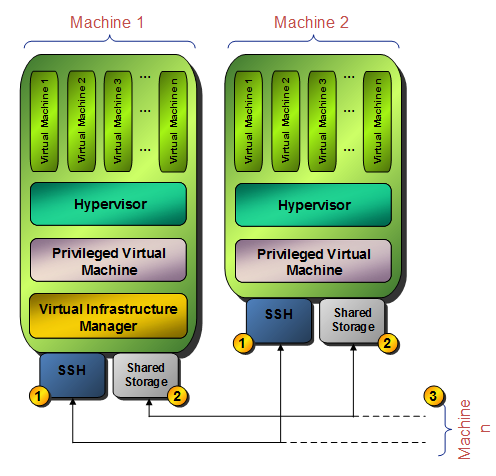
\includegraphics[scale=0.3]{cloudtestbed}}
\caption{Overview of the TestBed virtualised setup}
\end{figure}  

The current TestBed, consisting of 8 machines, uses OpenNebula, a competitor to OpenStack covered in the literature review of this report. However, in this project 2 machines have been allocated to this project and will use OpenStack to manage their resources as virtual infrastructure. 
Credit to Django Armstrong, who deployed OpenStack on the two machines in the Cloud TestBed for my use on this project, as I did not have the time or access privilege. 
These machines were accessed through the School of Computing network, using the machines Testgrid12 \& Testgrid13. The different projects such as Nova, Dashboard were available on different ports of this machine; e.g. port 443 for dashboard, \& port 5000 for Nova. This is in line with the general standard ports used in OpenStack\cite{openstackports}.  

\subsection{Experimenting with OpenStack - Experiment 0}
In order to learn how to interact effectively with OpenStack, I designed a first basic experiment which would require some interaction with at least 2 of its components. This experiment, as well as teaching me about OpenStack in general, would serve as a proof of concept for all future experiments, and provide examples of how to interact with OpenStack in 3 different ways, all of which may be used in future experiments; these are it's Web UI Dashboard, it's Command Line Interface, and it's Web Service APIs.\\
The experiment itself involves first authenticating a session via the OpenStack identity service, something which will be a prerequisite for almost every experiment, and to then perform a basic action using OpenStack compute, in this case creating a new Virtual Machine (VM) instance and starting it. In OpenStack, an instance is created from a template, known as an 'image' which is some configured software. I will introduce the chosen interaction method, describe how the experiment implementation was achieved in each case, and how they differed in approach, ease of use, and capability.  \\ 
The warm-up exercise described here can be found in Appendix E, and includes the results of each experiment, with details of the development environment(s) configured for this and further experiments.  

\section{Experiment Planning}

In order to get a good mix of Quantitative \& Qualitative evaluation, and to provide some useful practical information mixed with good coverage of OpenStack, the work to be done was set out as follows: 

\begin{itemize}
\item \textbf{Part 1: Architecture \& Feature Analysis of OpenStack} - Qualitative, descriptive analysis of the product. Overview of the product's design goals, choices, and its architectural characteristics will be provided, and an overview of the features of each component will be covered and explained, whilst being compared with the desirable and undesirable aspects of a cloud or VIM. 

\item \textbf{Part 2: Exploring OpenStack through Experimentation} - In this section of the report, several 'Experiments' will target specific functionality in OpenStack, and will demonstrate it through the use of RESTful APIs, CLI or Dashboard. Descriptions of the involved features and a review of their use will be given as a guide to using this functionality, as well as conclusions about the effectiveness of OpenStack's implementation. 

\item \textbf{Part 2b: Developing an OpenStack REST Client} - As previously mentioned as an aim of this project, a Java-based re-usable REST API client will be developed, in order to provide value to OpenStack users, and to perform experiments in part 2. This will be described in a separate appendix (E).
\end{itemize}

\section{Part 1: Analysis of OpenStack}

In this section, it is important to keep in mind the background research section of this report, specifically the 'Desirable Characteristics \& Challenges' of clouds and the 'Features of VIMs' section. The analysis below attempts to match OpenStack functionality to these factors to prove qualitatively that OpenStack is a valid and viable Cloud/VIM solution.  It will then go on to describe the benefits \& drawbacks of OpenStack functionality and features. 

\subsection{Architecture \& Feature Analysis of OpenStack}

The functionality of OpenStack is split into a number of different components, each of which are shown in the below figure detailing its architecture. Each component will be outlined in this section, along with its various notable features, uses and capabilities. It will then be analysed in terms of a number of basic metrics, including \textbf{coupling} and \textbf{cohesion}, and conclusions will be drawn about architectural choices. 

It is important to have a good understanding of the OpenStack offering so as to understand why it is good at what it does, how it deals with scale, and various other factors which determine whether it should be used for creating a Cloud.

\subsubsection{At a Glance}
\textbf{Introduction: }
Applications sit on top of OpenStack, utilising the infrastructure it provides via its APIS. This infrastructure is composed of Compute, Networking and Storage, all combined through OpenStack Shared Services, and accessed and managed via the OpenStack Dashboard. This allows the 'Cloud OS' openstack to be layered over commodity or standard hardware. Components each have their own REST APIs. 

\begin{figure}[H]
\centering
\fbox{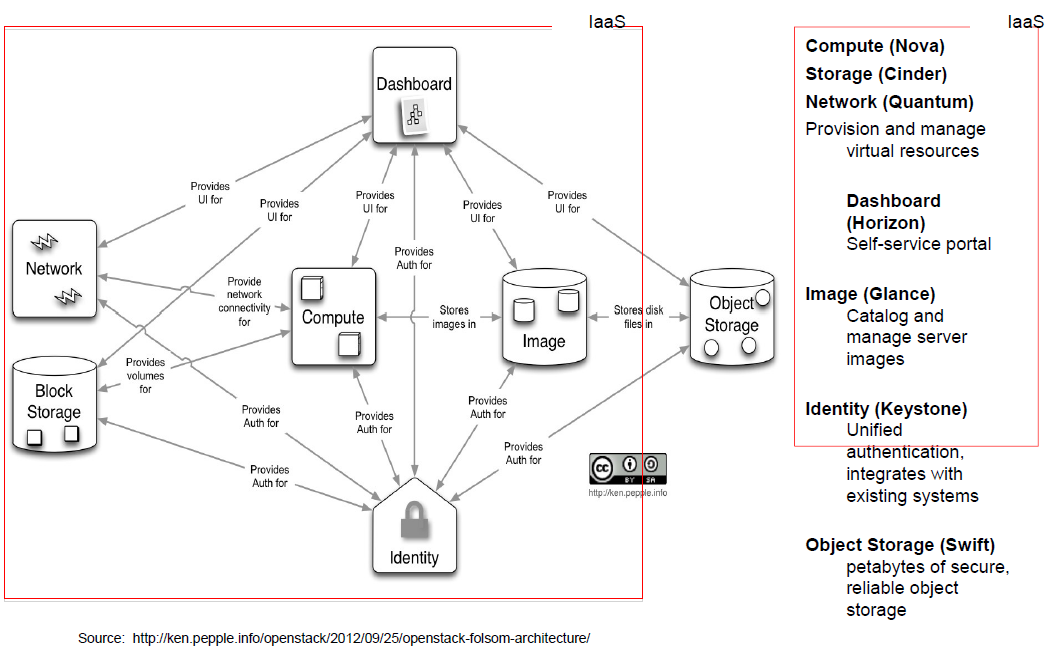
\includegraphics[scale=0.4]{openstack-architecture}}
\caption{Overview of OpenStack architecture \cite{openstacksoftware}.}
\end{figure}

\textbf{Analysis:}
The first noticeable feature of OpenStack's architecture is its number of distinct components, each of which interact with the others to provide Infrastructure as a Service. This is an interesting decision by the project designers, and differs greatly from similar projects such as OpenNebula. Conceptually, the design of OpenStack shows High Cohesion and Low Coupling. The functionality is split well into distinct blocks, each dedicated to a specific job, and handling, for the most part, only that job. The components communicate with each other through standards-compliant APIs in order to provide a fully functioning IaaS service. 

One considerable advantage of this approach, in line with the desirable aspects of a cloud discussed in chapter 2, is the level of customisation available to a consumer. Components can be left out, or even replaced with others, meaning that configurations of OpenStack are wide and varied, based on the needs of the users. In simple use cases, this can massively simplify the use and deployment of OpenStack, as only a small number of components need be configured, in turn saving on costs. Similarly, the approach effectively tackles one of the main challenges of the cloud - continuous evolution. When user requirements change, for example, more advanced networking is required, basic networking can be replaced with the neutron project. In this sense the 'cloud' need not be static. 
However, there may be some problems with this approach. Firstly, the level of complexity of communication is aptly displayed by the above figure; not only would this be difficult for professionals conceptually, but it could cause significant load, particularly on network performance, with so many distinct components constantly interacting. The issue of too much coupling and dependency in the system could also be a problem, if certain module dependencies are not fulfilled, such as Keystone for authenticating Nova requests. 

In terms of notable VIM features, OpenStack ticks many boxes. Virtual networking, storage, and dynamic resource allocation, and authentication are all provided by their own dedicated projects within OpenStack, meaning that, on paper, it really does satisfy most of the criteria for a working VIM. 

\subsubsection{Dashboard (Horizon)}

\textbf{Introduction:}
The OpenStack dashboard provides administrators and users a graphical interface to access, provision and automate cloud-based resources\cite{openstackdashboard}. It was designed in such a way that it can be combined with or used with third party services, such as those involved with billing, monitoring, or additional management. 

\textbf{Main Features:}
The dashboard is brandable, allowing users to make the tool available to its users in turn. The dashboard itself is a web application, and allows cloud administrators and users to control their compute, storage and networking resources. It also provides an overall view of the size and state of a cloud. Users and projects can be created, and users assigned to projects with set limits on the resources for those projects. Finally, and perhaps most notably, the dashboard offers users a self-service portal to provision their own resources within the limits set by administrators\cite{openstackdashboard}. This is one aspect of a cloud that we have established is very desirable. 

\textbf{Analysis:}
The first notable benefits of the Horizon project are its provision of a self-service portal for tenants in an IaaS cloud, which in turn allows the self-service provision of resources, one of the main desirable aspects of a cloud, and of a VIM. This is possible because the Dashboard allows simple interaction with the other OpenStack projects, such as Nova, which handles resource provision. 
Another key point aspect of clouds provided by Dashboard is accessibility; it can be securely accessed over a network connection, and so reliable accessibility is possible. 
By far the most distinctive aspect of the component is the gradual learning curve it provides. For me personally, many of the concepts regarding OpenStack were learned through using the Web UI, as it is informative, and extremely simple to use. This in turn gives users a much better grasp of OpenStack as a whole. 
 
The level of integration offered by Dashboard is unparalleled across the OpenStack offering, and it is in fact difficult to see which project is being used at times, due to the abstract nature of User Interfaces. This fact can be both a blessing and a curse; it is good for a user to focus on the task at hand, and not have to worry about disparate functionality, but it is also difficult to spot which components are used more than others, or even whether some are necessary. The level of information given on project components is good using Dashboard, and this goes some way to solving this issue. 
One problem I did spot when using Dashboard, and leading on from the abstraction mentioned, is that it uses naming often inconsistent with other parts of OpenStack. For example, 'instances' are managed using the Dashboard, where the equivalent Nova API calls would handle 'servers'. This is a subtle difference, but can be extremely confusing for users. 

\subsubsection{Compute (Nova)}

\textbf{Introduction:}
The Compute part of OpenStack allows a business or other user to offer on-demand computing resources, by provisioning and managing large networks of virtual machines. Compute resources are accessible via APIs for developers building cloud applications and via web interfaces for administrators and users\cite{openstackcompute}. It is designed to scale horizontally as new hardware is added. 
Both KVM and XenServer hypervisors are available to use with OpenStack, although other hypervisors are also available;  Linux container technology such as LXC is also supported for scenarios where users wish to minimize virtualization overhead and achieve greater efficiency and performance. In addition to different hypervisors, OpenStack supports ARM and alternative hardware architectures\cite{openstackcompute}. \\
Popular use cases of this component include offering IaaS compute further up the stack, processing big data with tools such as Hadoop, scaling compute to meet unpredictable demand, and HPC elements with diverse and intensive workloads. 

\textbf{Main Features:} 
Notable features of Compute include\cite{openstackcompute}:
\begin{itemize}
\itemsep0em
\item Management of virtualized server resources such as
CPU, memory, and network interfaces.
\item Manage Local Area Networks (LAN)
\item Virtual Machine (VM) image management, and live VM management.
\item Store and Manage files programmatically via API
\item VM Image Caching on compute nodes for faster provisioning of VMs.
\end{itemize}

\textbf{Analysis: }
Nova is the 'bread and butter' of OpenStack as a Virtual Infrastructure Manager. It provides a number of key cloud characteristics, such as virtualisation support, elasticity of resources, and effective resource allocation. 
The ability to access nova via the command line, REST APIs and the Dashboard means that it provides accessible, self-service resource provisioning for the full VM lifecycle.  
Flavors, a concept introduced in the warmup exercises, allow for servers to be built at different sizes, and even running servers can be rebuilt at different resource sizes, giving a great level of elasticity. The ability to launch new servers from either images, i.e. bootable files, and snapshots of servers hugely accelerates the use and simplicity of the Nova functionality. Server migration offers efficient allocation of virtual resources, and Nova can even decide automatically the best server to migrate a server to. Aside from this, detailed information on resources is provided using Nova, meaning management of resources is very simple. 

Clearly, we can see that Nova provides all the functionality it takes to run an Infrastructure cloud. There were some problems I noticed, however, with the design of this component. As Nova is so important, it appears that concepts from other projects have been 'borrowed' so as to allow no dependence on other projects, such as the Glance Image service. This points to low cohesion, where the functionality of the Nova API can often seem out of place - it appears that nova tries to 'do it all' with concepts of images, networks, and flavors in it's API. Not only does this make for a badly designed API, but it can confuse users when trying to use Nova with other components, or even make other components redundant. 

\subsubsection{Networking (Neutron)}

\textbf{Introduction:}
OpenStack Networking is a pluggable, scalable and API-driven system for managing networks and IP addresses. It ensures the network will not be the bottleneck or limiting factor in a cloud deployment and gives users real self service, even over their network configurations\cite{openstacknetwork}.

\textbf{Main Features:}
The notable capabilities of Networking include\cite{openstacknetwork}: 
\begin{itemize}
\itemsep0em
\item flexible networking models e.g. flat networks or VLANs for separation of servers \& traffic.
\item manages IP addresses, allowing for dedicated static IPs or DHCP. 
\item Users can create their own networks, control traffic and connect servers to networks.
\item Administrators can take advantage of software-defined networking (SDN) technology.
\item extension framework allowing additional network services.
\end{itemize}

\textbf{Analysis: }
The feature list for the Neutron project is very impressive. The provision of Virtual networking is an essential for a VIM, and the ability to make use of the very important Software Defined Networking (SDN) technology shows that Neutron is very advanced in this area. Neutron provides a good level of customisation, allowing for flexible alternative networking models which make it ideal for adapting to changing user requirements. Users can self-serve using this functionality, and scale it down elastically with compute resources, making it a perfect partner for the Nova project. 

Neutron is a highly cohesive module; all functionality is dedicated to the management and maintenance of networking between compute instances, and the number of options within this is staggering. There are a number of extensions to this which provide added functionality, some of which appear to 'belong' to the module less, such as quota management for network resources. This is inconsistent with quotas for compute resources, which are not handled by the Nova API in this way.  

One issue with Neutron is its complexity. It appears that a 'default' simple configuration is hard to come by, and it has a steep learning curve. This is perhaps another reason that simpler functionality is available from the Nova project, to reduce dependence on the Neutron project to those only requiring advanced configurations. Perhaps it would make more sense for this to be split into basic and advanced networking features, but the 'extensions' design model seen across OpenStack projects sees well to this aim. 

\subsubsection{Block Storage (Cinder)}
\textbf{Introduction:}
 "\textit{ Block Storage allows block devices to be exposed and connected to compute instances for expanded storage, better performance and integration with enterprise storage platforms, such as NetApp, Nexenta and SolidFire}"\cite{openstackstorage}.

\textbf{Main Features:}
Block storage offers the following notable capabilities\cite{openstackstorage}:
\begin{itemize}
\itemsep0em
\item provides persistent block level storage devices for use with OpenStack compute instances.
\item block storage system manages the creation, attaching and detaching of the block devices to servers.
\item Unified storage support for numerous storage platforms 
\item Snapshot management for backing up data stored on block storage volumes. 
\end{itemize}

\textbf{Analysis: }
Cinder's block storage provides a fully integrated service to the Nova compute project, providing scalable, flexible storage that acts as an extension to server instances. The provision of Storage virtualisation is deemed a very important aspect of functionality for a VIM, as uncovered by the research section of this report. The ability to scale up and down these block devices provides a seemingly ever-present flexibility and customisation for provisioning resources.
The Cinder project has a good level of integration with the other projects, such as Nova \& Dashboard, whilst maintaining no dependency on either. Integration with third party storage platforms further shows the level of capability of Cinder. Functionality from the project is very well split, even being distinct from object storage, which has a different task and uses a different storage type. This is one area where the design of OpenStack is very well thought out. 
Cinder has the benefit of being able to run on commodity hardware, something it has in common with many of the projects across OpenStack. For storage in particular, this is a great saver on costs, something which is very desirable for an IaaS cloud. Snapshot capability also greatly improves the reliability of Servers through backups, and accelerates the deployment of Server VMs in the data centre. 
 
One issue which has become apparent for Cinder is the extra configuration needed to run it. This is something that Django ran in to personally when deploying OpenStack for this project. It appears the Logical Volume Management (LVM) is required to run Cinder, and this is not clear in the documentation for the project, a potential cause of problems for some administrators.
 
\subsubsection{Object Storage (Swift)}
\textbf{Introduction:}
"\textit{Object Storage is ideal for cost effective, scale-out storage. It provides a fully distributed, API-accessible storage platform that can be integrated directly into applications or used for backup, archiving and data retention. }\cite{openstackstorage}:.

\textbf{Main Features:}
Object storage offers the following notable capabilities\cite{openstackstorage}:

\begin{itemize}
\itemsep0em
\item redundant, scalable object storage using clusters of standardized servers capable of storing petabytes of data
\item not a traditional file system, but rather a distributed storage system for static data such as virtual machine images, photo storage, email storage, backups and archives. Having no central "brain" or master point of control provides greater scalability, redundancy and durability.
\item OpenStack software responsible for ensuring data replication and integrity across the cluster.
\item Storage clusters scale horizontally simply by adding new servers. Should a server or hard drive fail, OpenStack replicates its content from other active nodes to new locations in the cluster. 
\end{itemize}

\textbf{Analysis: }
Swift provides some essential beneficial cloud characteristics. As is mentioned above, it provides redundancy, scalability and durability. Swift is the project which ensures data is not lost, that replication is managed efficiently, and that storage cluster use is extremely scalable. Along with Cinder, it provides the essential storage virtualisation capability that every VIM needs, but is instead a distributed filesystem for storage of OpenStack files, not just for consumption by Server VMs. Swift appears to be the backbone of an OpenStack cloud. It manages disaster recovery, reliability and availability of data. 
Based on the differences noted between Swift and Cinder, the designers made a good choice in keeping this functionality separate, even though it seems conceptually similar. 

In terms of cohesion, swift is a well designed module. The 'object' storage approach keeps working with Swift very abstract, and so it covers a wide range of different entities, whilst keeping the same work flow conceptually. 

One odd design choice is that Swift has its own concept of 'account' management to handle which storage belongs to which users. It would seem that this would be more appropriate in the Keystone project, which manages identity, but this may just be another example of the duplication seen across OpenStack to maintain its loosely coupled architecture. 

\subsubsection{Identity Service (Keystone)}
\textbf{Introduction:}
The first shared service, \textbf{OpenStack identity}, provides a central directory of users mapped to the OpenStack services they can access. It acts as a common authentication system across the cloud operating system and can integrate with existing backend directory services like LDAP. Additionally, the catalog 
provides a queryable list of all of the services deployed in an OpenStack cloud in a single registry. Users and third-party tools can programmatically determine which resources they can access. 

\textbf{Main Features:}
Aside from basic authentication services, Keystone offers the following services.
For administrators, identity allows configurations of policies concerning users and groups, creation of users and permissions management for other components, and integration with services such as LDAP. For users, lists of accessible services and logging of API requests per user are provided. 

\textbf{Analysis:}
Keystone's first obvious key characteristic is security; security is of paramount importance in any multi-tenant system, especially due to the remote nature of clouds. Keystone not only provides this security for the UI dashboard, but also for every other service in OpenStack, such as Nova or Glance. This makes Keystone extremely important in any deployment. Keystone is very customisable, providing integration with services such as LDAP, and identity management, including 'groups' of users and user based 'projects'. 
The token-based authentication method employed by Keystone is incredibly easy to use, especially in terms of development using its REST API. It is important that something as important as security be simple to employ, as it leaves less room for error. 

Keystone is arguably the most highly cohesive module in OpenStack. It is very specialised, and an archetypal use of the 'loosely coupled' mantra. It provides a clearly defined service for every other module, and this design makes a lot of sense. This pattern of having identity stored in one place used for all is common across modern applications, for example Google's single sign on system, which is the same for Google Docs \& Google Mail\cite{googleapps}. 

However, there could be some issues caused by Keystone. Firstly, it represents a single point of failure in terms of security; if it is compromised, every single service becomes compromised. Secondly, it is likely that network overhead could be much higher, as conceptually, every time a request is sent to a project like Nova, it must use Keystone remotely to validate the supplied authentication token. This adds one extra request to every request sent by a client, which would scale with the number of requests sent. 
The final issue, which is more abstract, is that Keystone's necessity arguably goes against the loosely coupled design of OpenStack. One of the advantages of the design is that some modules can be left out and OpenStack can still run, but of course, Openstack cannot be run without Keystone securely.

\subsubsection{Image Service (Glance)}
\textbf{Introduction:}
The \textbf{OpenStack Image Service}, provides discovery, registration and delivery services for disk and server images, as well as snapshotting functionality. The Image Service can store disk and server images in a variety of back-ends, including OpenStack Object Storage.  The Image Service API provides a standard REST interface for querying information about disk images and lets clients stream the images to new servers.

\textbf{Main Features:}
Capabilities include allowing admins to create templates for compute instances, allowing users to choose from available images, or create their own from existing servers. Snapshots can also be stored in the Image Service to that they can be backed up quickly. 

\textbf{Analysis:}
Glance offers the benefit of simplified application accelleration. The provision of 
bootable virtual machine images means that Servers can be deployed extremely quickly, and with minimal work from the client, which simply chooses a VM size and an image, with OpenStack handling everything else. 
Glance is not a very large component, and so is likely to be cohesive. One issue with its design I have discovered is the ambiguous part-inclusion of VM snapshots into Glance. A Snapshot is a capturing of the state of a Server, which can be used to launch new Virtual Servers of the same state. Snapshots should arguably be in Glance, as they are very similar to images, but are in fact handled in the Cinder component. They can however be stored and backed up with Glance; this is something that may cause a lot of confusion, and certainly couples cinder and glance together, something against the design ethos of OpenStack.


\section{Part 2: Exploring OpenStack through Experimentation}

\subsection{Introduction}
In this section, a number of experiments are performed on certain components of OpenStack, to provide some useful information about it in terms of function and performance. 

The main types of experiment include:
\begin{itemize}
\itemsep0em
\item Validation Experiments - aimed at simply exhibiting OpenStack functionality; using it for its intended purpose, showing that it works, and providing re-usable code so that it can be performed on other OpenStack configurations. They will target a subset of functionality for a given project component. 
\item Performance Experiments - will attempt to time operations using OpenStack. Due to lack of comparison with other products, the idea will usually be to compare different parts of OpenStack to eachother. For example, comparing the cost of starting different sized VMs shows how size affects performance, and this is useful, Quantitative Evaluation. 
\item Other Experiments - will perform some actions on OpenStack and attempt to validate or nullify a hypothesis, in a way which will shed some light on the workings of OpenStack. 
\end{itemize}

The OpenStack components highlighted for these experiments are Nova \& Keystone. The reasons for other components not being included is included in the Evaluation section of this report. 

\textbf{Images \& Flavors:}\\
The concept of Images, used by Nova \& Glance, i.e. files containing bootable data used to launch Virtual Machines, or servers, and of Flavors, i.e. 'sizes' of a Virtual Machine in terms of its resources, have been introduced in Appendix E, the 'warmup exercises'. Nevertheless, it is important to introduce the Flavors and Images used in the following experiments. \\
Only one image is used in all the experiments: 
\begin{itemize}
\item Name: Cirros 0.3.1 Size: 12.5 MB. This image was already on OpenStack when I began to use it, and is used consistently for each relevant experiment. 
\end{itemize}

The flavors being used are:
\begin{itemize}
\item Name: m1.tiny   VCPUs: 1 Disk Capacity: 1GB  RAM: 512MB
\item Name: m1.small  VCPUs: 1 Disk Capacity: 20GB RAM: 2048MB
\item Name: m1.medium VCPUs: 2 Disk Capacity: 40GB RAM: 4096MB
\end{itemize}

Knowing these sizes is very important for understanding results from some of the experiments in this section. 

\subsection{Keystone}

\subsubsection{Experiment K1: Keystone Validation}
\textbf{Introduction:}
This experiment will target key functionality of the Keystone Identity Service, exhibit it, and provide a Java API for other clients to easily interact with the service via it's RESTful Web Service. 

\textbf{Aims, Considerations \& Metrics:}
The main aim of this experiment is to validate the functionality of Keystone, particularly on the cloud testbed. The functionality of Keystone of interest includes:

\begin{itemize}
\itemsep0em
\item Generating an Authentication Token
\item List tenants that can use a particular Token
\end{itemize}

The main considerations with this experiment will be those related to the architecture of the OpenStack client \& Experiment framework deliverable of this project. There should be an easy way to obtain an authentication token, and use this with other services. 
The main metrics in play with a validator experiment will be the complexity of the API conceptually, and the complexity of the Client code developed subsequently. 

\textbf{Experiment Steps:}
Step 1 will be to develop a Java interface representing the functionality that should be produced as part of the delivered OpenStack client \& Experiment framework. Once created, this will then be implemented using Spring's RestTemplate to fire requests to the given OpenStack setup. 
An Experiment class will then be developed to consume it through the aforementioned interface, and demonstrate its effectiveness.  
Finally, decisions will be made on how to structure the obtaining of authentication tokens to ensure an elegant client process. 

\textbf{Development \& Execution:}
The first decision made, as part of the development of an authentication mechanism for the client was to use version 2 of the Keystone API, mainly for consistency with other APIs \& simplicity of functionality, considering basic authentication is all that is required. 

\textbf{\textit{Part 1: Generating an Authentication Token}}
Generating an authentication token using the REST API is achieved through the following steps, based on the Keystone API reference Documentation: \cite{keystoneref}

\begin{itemize}
\itemsep0em
 \item The Client sends a POST request to \url{http://OPENSTACK_URL:5000/v2.0/tokens/}.
 \item Keystone responds with a character string known as an Authentication Token. 
 \item This token is included in the headers of subsequent requests which require authentication as the field "X-Auth-Token".
\end{itemize} 

This particular functionality was developed as part of the warm up exercises, which can be found in Appendix E. The code fires a POST request containing authentication information, and if this information is valid, the response body contains a valid authentication token. 
In order to test this token works, the Nova Client from Experiments N* and the warmup exercises in Appendix E will be used to perform an action which requires authentication. In this case, that will be the method \textit{getImageInfo}. This will be introduced in later experiments, but for the intents of this experiment, it is sufficient to know that it requires authentication.  

\textbf{\textit{Part 2: Listing Tenants of a particular Token}} 
This piece of functionality aims at telling the user which tenants are authenticated via the given token. A good use case of this, for example, is finding out whether one user has admin privileges, or even whether the given token can be used by a particular user. 
Development started by assessing the arguments which were sent back and forth. A GET request should be sent to \url{http://OPENSTACK_URL:5000/v2.0/tenants/} with the header field 'X-Auth-Token', containing the token which should be analysed by Keystone. \\
In response to this, Keystone sends a JSON representation of a number of 'Tenants', synonymous with users in OpenStack. 
The class \textit{Tenant.java} was created to store the information on each tenant, and these can be returned to the client directly, with each field accessible through getter methods. 
 
\textbf{Results:}
The resulting log file can be found in Appendix F, and in the file \textit{K1-results.log} in the logs/ directory of the final deliverable of this project. 
Overall, the experiment was a success. The interface \textit{KeystoneClient} was used to access its implementation, \textit{KeystoneClientImpl}, and the two methods \textit{authenticate} and \textit{listTokenTenants} were successfully called and validated. 
A call to the Nova Client to assess the validity of the given token was also performed successfully, and the design of the client mechanism for authenticating requests was subsequently designed; this will be covered in the conclusion to this experiment. 

\textbf{Conclusion:}
Authentication is kept extremely simple in OpenStack, and this makes it very easy to use. This experiment has demonstrated how a single request can be used to obtain a token with which further requests can be made. This is elegantly achieved through HTTP headers, an easy to use and robust form of message authentication.  
Through the newly developed \textit{KeystoneClientImpl} implementation, other Java class clients can now easily authenticate with OpenStack. 
The main design decision that came out of this experiment was that each subsequent client requiring authentication would have the token saved as a field, set through a mandatory \textit{setAuthToken} method. 

\textbf{Resources:}
NovaClient.java
KeystoneClient.java
KeystoneClientImpl.java
KeystoneValidatorExperiment.java
Tenant.java


\subsubsection{Experiment K2: Packet Interception}
\textbf{Introduction:}
This experiment should confirm that authenticating with OpenStack via Keystone is safe. Authentication is an extremely important part of using any multi-tenant service, as intrusion could disrupt the running of an entire business, or leak very sensitive data. 
One way of gaining such access is through the interception of packets containing authentication data, and using this information to authenticate actions on OpenStack.

\textbf{Aims, Considerations \& Metrics:}
The idea behind this experiment is to attempt to exploit the fact that authentication requests are sent over the network via HTTP, and intercept the request or the response. If and when the packets containing this information are found, the level of information available to someone snooping packets will be discussed, and if the token itself is discernible, it will be used to perform subsequent requests which require authentication, for example, terminating a Server. 
I expect this experiment to fail, as there should be some mechanism of security in OpenStack. Nevertheless, it is useful to find out just how much information is actually exposed from an authentication handshake. 

\textbf{Experiment Steps:}
The first step in this experiment is to write a very basic Java Experiment for the REST API, which would simply get an authentication token using the Keystone API \& display this for the user. Knowing this token is a way of knowing what to look for in packets being intercepted. 
The next stage is to find some tool to intercept \& analyse network traffic. I decided to install the free, open source packet analyser Wireshark\cite{wireshark} on my personal machine, connected to OpenStack via SSH tunnelling. This tool allows the analysis of packets from any given network interface, and provides a sophisticated packet filtering tool. 

Once these are in place, the experiment steps are as follows:
\begin{itemize}
\itemsep0em
\item Configure Wireshark to analyse main network interface on personal laptop
\item Perform Simple Auth Experiment to get an auth token, and retrieve token.
\item Perform a number of filters on packets using Wireshark to attempt to find them, \& if found, extract information from them.
\item If any information is found, report this, and if enough to be useful, attempt to use it to authenticate a new task using the Nova compute project. 
\end{itemize} 

\textbf{Development \& Execution:}
\textbf{\textit{Part 1: Develop a Simple Authentication Experiment}}
This part of the development was very straightforward. The functionality was described in Experiment K1, and the first part of that experiment, which performs simple authentication, was moved into a separate experiment which would print information about the token. This can be found in the \textit{SimpleKeystoneAuthenticationExperiment} class. 

\textbf{\textit{Part 2: Install \& Configure Wireshark}}
Installation of WireShark was also a straightforward process. As I was using Ubuntu Linux, I used the aptitude package manager\cite{aptitude} to downloads page\cite{wireshark} and a simple step by step process automatically installed it.
The next step was to get WireShark up and running. This is achieved through choosing a network interface from the home screen. I selected the interface lo, i.e. the loopback interface, and connected to the Leeds test bed via Putty\cite{putty} using port forwarding from this loopback, or 'localhost'. This gave me the following network analysis view, containing all packets sent to and from my personal machine connected to OpenStack via localhost urls:

\begin{figure}[H]
\centering
\fbox{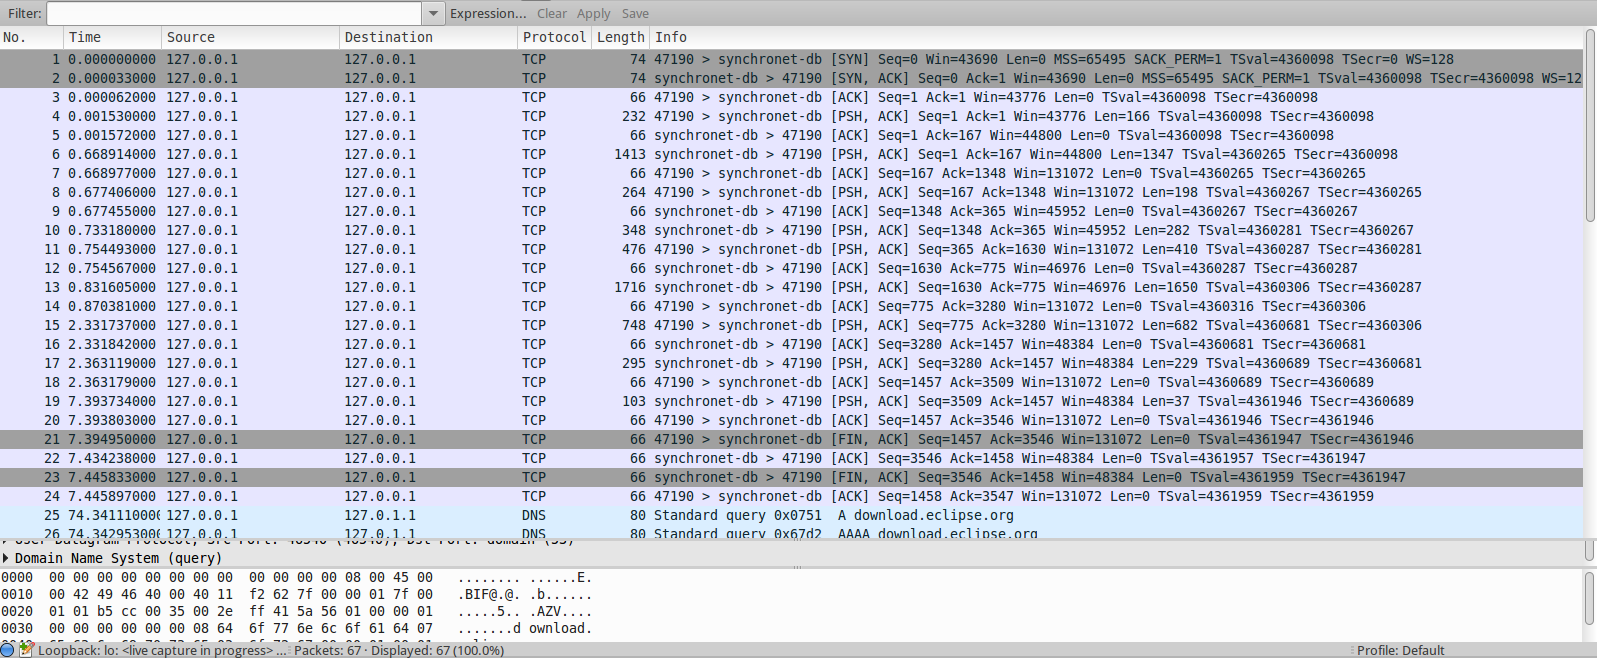
\includegraphics[scale=0.27]{wiresharknetanalysis}}
\caption{WireShark Packet Analysis View}
\end{figure}

\textbf{\textit{Part 3: Develop tailored searches for authentication packets}}
In order to attempt to find the packets responsible for transferring data, the WireShark packet filtering tool will be used. This allows a search query to be entered to filter packets, similar to regular expressions. 
If it is not possible to use this to pick up the packets, then the information is not accessible via intercepting packets, at least not through these means, which implies that it is safe.

The main search queries used will be:
\begin{itemize}
\item Search for requests sent to port 5000 (keystone port):    '\textit{tcp.port eq 5000}' 
\item Search for the Auth Token given from experiment: '\textit{http contains TOKEN}' 
\item Search for header identifier 'X-Auth-Token':      '\textit{http contains "X-Auth-Token"}'
\end{itemize} 

Executing the experiment is simple; for each of the above queries, apply the filter to WireShark, then run the aforementioned Keystone Experiment which authenticates. 

\textbf{Results:} 
Running the first query, as shown in the below figure, returned all the relevant packets first time. 
\begin{figure}[H]
\centering
\fbox{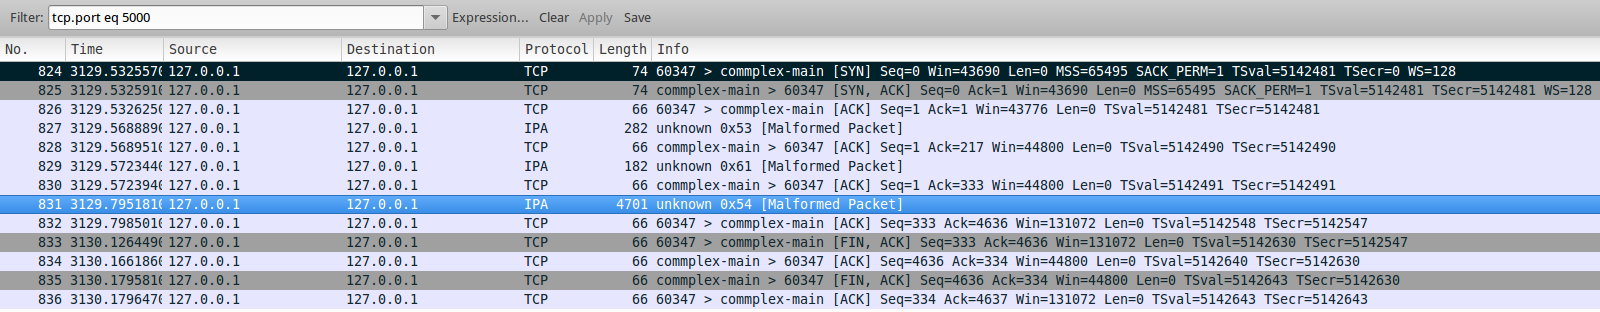
\includegraphics[scale=0.27]{keystone-packet-returned}}
\caption{WireShark Packet Analysis Query results}
\end{figure}

The outcome of this experiment was surprising. As it is possible, and generally default behaviour to run Keystone over HTTP and not HTTPS, it was possible to extract all of the data sent back and forth by the REST Client. This data was extracted using wireshark's 'copy -> bytes -> printable text only' option on the packets, and can be found in the file \textit{extracted-packet-text.txt} in the /logs directory of the final submission. Data captured included username, password, and the returned token, which was then used with the Advanced Rest Client introduced in Appendix E to confirm its validity, shown below: 
\begin{figure}[H]
\centering
\fbox{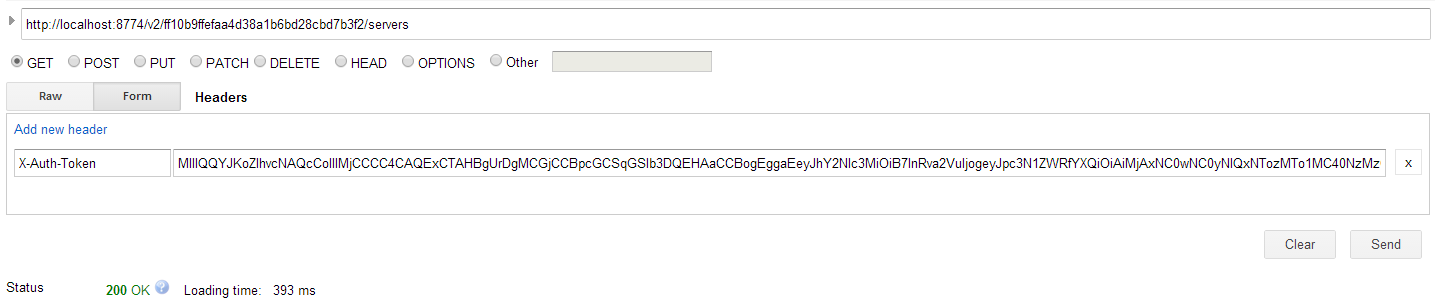
\includegraphics[scale=0.3]{arc-keystone-packet}}
\caption{Running the Advanced Rest Client with the extracted Auth token successfully}
\end{figure}

\textbf{Conclusion:}
In conclusion, it is clear that there is a real problem with security if the administrator does not choose to use HTTPS to communicate with the OpenStack Keystone service. In my personal experience with a similar product, HTTPS was enforced as there does not seem to be a use case where security of an authentication project would not be paramount. It is imperative that any OpenStack deployment used in the real world be configured to use HTTPS, which would not expose this level of information. This is the same for any web site or endpoint using HTTP. 

\textbf{Resources:}
\textit{SimpleKeystoneAuthenticationExperiment.java}
\textit{extracted-packet-text.txt}



\subsection{Nova}

\subsubsection{Experiment N1: Nova Validation}

\textbf{Introduction:}
This experiment will target key functionality of the Nova Compute service, exhibit that functionality, and provide a Java API for other clients to easily interact with the service via its Restful Web Service. 

\textbf{Aims, Considerations \& Metrics:}
The main aim of this experiment is to validate the functionality of Nova, in particular on the cloud testbed. The functionality of Nova of interest includes:

\begin{itemize}
\itemsep0em
\item Creating \& Deleting Servers
\item Obtaining Information on Servers, Flavors \& Images
\item Managing Server \& Image Metadata
\item Rebooting Servers
\item Changing the password of a Server
\end{itemize}

This part of OpenStack is of the utmost importance, as it is core functionality. It will therefore be by far the largest client available, and so will include the largest subset of available functionality, and have the most experiments based upon it. 

The main metrics involved will be a review of the process of developing a client, whether the concepts are too complicated, or whether they could be improved. 

\textbf{Experiment Steps:}
The experiment itself involved a number of large steps, and a number of smaller steps for each of these. The basic development model at a high level was as follows:

\begin{itemize}
\item Identify desirable functionality of Nova via the API reference (v2) \cite{novaref}
\item Using this reference, identify the action required to perform this functionality via REST.
\item Develop the client code to perform this action. 
\item Add this action to the Validator Experiment and run it. 
\item Review the functionality via qualitative metrics such as ease of use, coherency, complexity of client code, etc.
\end{itemize}


\textbf{Development \& Execution:}
The functionality listed above was extracted from the Nova API reference, and an interface \textit{NovaClient} was created to represent this locally. Broadly, this functionality was split into three main groups; Information retrieval, server actions, \& metadata actions. Note, all of these actions require authentication headers mentions in experiment K1. 

\textbf{\textit{Part 1: Information Retrieval}}
This section concerns a number of methods to obtain information about Servers, Images, and Flavors, also referred to here as 'entitites', introduced earlier in this report. Information on these is required to perform any useful action with the Nova project. 
The nova project has a 2-tier pattern for retrieving information in this way. Firstly, there are actions which will retrieve basic information about an entity (i.e. server), usually limited to names, ids and url references. This information can be used to retrieve more detailed information about these entities, for example, getting a server by its id. Nova also provides a method for retrieving details of all the entities of a given type. 
To represent this in Java, the decision was made to design two Java classes to represent each entity. The basic info would be called ENTITYInfo.class, i.e. \textit{ServerInfo}, \textit{ImageInfo}, \textit{FlavorInfo}. The more detailed information, in line with Object Oriented principles, would simply be named for the entity, i.e. \textit{Server}, \textit{Image}, \textit{Flavor}. 
Retrieving this information is performed with GET requests. After the base URL %\begin{verbatim}
\url{http://OPENSTACK_URL:8774/v2/TENANT_ID/}
%\end{verbatim} 
the url extension flavors, servers or images can be used to 'get' basic information on all of these. Further adding 'detail' to the URL provides a similar retrieval of all, and adding a specific id, be it server, image, or flavor, allows a 'get' to retrieve details on a given entity.  

\textbf{\textit{Part 2: Server Actions}}
Nova allows for a number of actions on a server. Firstly, and arguably most importantly, is the creation of a Server. This is achieved by sending a POST request to the URL 
\url{http://OPENSTACK_URL:8774/v2/TENANT_ID/servers},
supplying a reference link for an Image and for a Flavor, described in the previous part.  This creates a server, returning information about the newly created server. 
Deleting a server is as simple as sending a DELETE request to the above link with '/SERVER\_ID' appended. 
The other two actions require sending POST requests to the URL 
\url{http://OPENSTACK_URL:8774/v2/​{tenant_id}​/servers/​{server_id}​/action}.
For rebooting, a simple request body containing the word 'reboot' is sufficient, but for changing a password a new password must be supplied.  

\textbf{\textit{Part 3: Metadata Actions}}
Metadata is extra information that can be added to an Image or a Server using Nova. This information is stored as a simple key-value collection. 
This is very simply retrieved and modified on a per-entity basis. 
Firstly, performing a GET request on the URL 
\url{http://OPENSTACK_URL:8774/v2/TENANT_ID/SERVERS_OR_IMAGES/ENTITY_ID/metadata}
will return each key value pair, and sending metadata in a POST request would update these. Issuing a GET, PUT or DELETE request to this URL plus '/KEY' allows for retrieval, updating or deleting of a specific value by key. 
In java, metadata is represented using the \textit{Map} class from Java's Collections library.
All of this functionality was developed and can be found in the class \textit{NovaClientImpl}, and an experiment using this client was developed, called \textit{NovaValidatorExperiment}. This experiment performs checks that functionality does exactly what is described.  
 
\textbf{Results:} The resulting log file for the experiment can be found in the file \textit{NovaValidatorExperiment.log}. Overall, the experiment was a success. The interface functionality was validated, and a reusable client developed for further use. 

\textbf{Conclusion:} Nova functionality is varied and powerful. From performing asynchronous server operations, to gaining quick access to information regarding resources in OpenStack, the REST API is a useful tool with a logical RESTful request structure. Having the concept of images and flavors in Nova also greatly simplifies the process of performing cross-conceptual tasks such as creating a server from a specified image.
One issue uncovered was the inconsistent representations of entities in JSON format, causing problems for a client. For example, there are 3 different representations of a Server; one with basic information, one with details, and one given after a new server is created. This can become extremely confusing. Similarly, problems were uncovered with timing when no clear indication of job completion or status is given. This was remedied with a number of Utilities, found in the \textit{NovaUtilities} class. 

\textbf{Resources:} \textit{NovaValidatorExperiment} \textit{NovaClient} \textit{NovaClientImpl} \textit{NovaUtils}

\subsubsection{Experiment N2: Nova Extensions Validation}

\textbf{Introduction:} In a similar fashion to the previous experiment, this will target functionality that is part of the Nova 'Extensions API'; this represents functionality above and beyond normal Compute tasks, usually requiring Administrative privileges. The experiment will exhibit this functionality, and provide a means for other clients to do so too. 

\textbf{Aims, Considerations \& Metrics:}
The subset of functionality that is of interest to this project includes:

	\begin{itemize}
	\itemsep0em
	\item Suspend, Resume, Pause, Unpause, Lock, Unlock actions on a Server
	\item Obtaining information on Physical Hosts 
	\end{itemize}

This is mainly due to what the following experiments will aim to achieve, and what tasks are most commonly performed in a virtual infrastructure solution. 
One other consideration will be accessing the extensions API, and whether it should be distinct from the original Nova API Client in the Java Client solution.
Similarly to the previous 'validators', the main points of measurement will involve conceptual complexity of the API, and the code developed to make use of it. 

\textbf{Experiment Steps:}
Following a similar pattern to the previous experiment, the idea is to develop a Java interface for the extensions client \& then implement this using a REST service client. 
Next, an Experiment class will be developed to exhibit this functionality, in order to allow me to form conclusions about the API, and validate its effectiveness on the Cloud testbed.
 
\textbf{Development \& Execution:} In creating a Java interface \textit{NovaExtensionsClient}, the first decision was to link this client to the original Nova client. This is mainly to keep in with the conceptual 'extension' relationship between the two, and because it is likely that the implementations of each will be very similar (e.g. if one is a spring rest client, the other is likely to be too). A method \textit{getNovaExtensionsClient} was added to the \textit{NovaClient} interface to allow this coupling. 
Next, the functionality was tackled in 2 parts.

\textbf{\textit{Part 1: Admin Server Actions}}
Firstly, there are a number of actions that can be performed on a server, such as locking, suspending, or pausing. These all cause the \textit{status} of the Server to change. More information on these statuses can be found in OpenStack's Documentation, specifically in the List Server manual\cite{osserverstatus}.
Developing the requests for each of these, based on the nova extensions API reference \cite{novaextref}, is relatively simple, as they take the following simple JSON form: 
\begin{verbatim}
{
	"ACTION" : "null"
}
\end{verbatim}
where action is the action, such as 'lock' or 'pause'. 
These requests are sent to the URL \url{http://OPENSTACK_URL:8774/​TENANT_ID​/servers/​SERVER_ID​/action} and return no response.

\textbf{\textit{Part 2: Obtaining Host Information}}
Obtaining information about a physical Host can be achieved in 2 ways using the Nova Extensions API. The first of these is to list all Hosts running OpenStack that the tenant can access; this is achieved by sending a GET request to the URL:
	\url{http://OPENSTACK_URL:8774/TENANT_ID/os-hosts}
From this request, a JSON response containing basic information about each host, such as host name, is returned. In order to handle this response, the \textit{HostInfo} class was created. 
The second form of Host information retrieval is achieved by querying one specific Host, usually retrieved with the first technique discussed above. A GET request is sent to the URL :
	\url{http://OPENSTACK_URL:8774/TENANT_ID/os-hosts/HOST_NAME}
	
and this returns a more detailed summary of a Host, defined as a collection of 'Resources' such as CPU. To represent this in Java, a \textit{Host} and \textit{Resource} class was created, with the former containing a List of the latter.  
Note that the use of \textit{HostInfo} and \textit{Host} as two different levels of detail is a pattern that is kept consistent with those mentioned in experiment N1, in order to avoid confusion and make clear the levels of information given. 

\textbf{Results:} The resulting log file can be found in the file \textit{NovaExtensionsValidatorExperiment.log}. The experiment was successful, and functionality was successfully validated. 
\textbf{Conclusion:} The Nova extensions API provides extra functionality which is essential for any advanced Compute setup. In particular, the state change of a Server, such as Suspending or Pausing, allows for a good level of Server manipulation, meaning that resources can be more effectively managed. One piece of functionality that was unable to be used due to a hardware limitation was server migration, but this is indeed part of the Extensions API. 
\textbf{Resources:}  \textit{NovaExtensionsValidatorExperiment.log}, \textit{NovaExtensionsClient}, \textit{NovaExtensionsClientImpl}, \textit{NovaUtils}

\subsubsection{Experiment N3: Server Launch Performance}

\textbf{Introduction:}
This experiment is centred around a very important part of core OpenStack functionality; the launching of Virtual Servers, i.e. Virtual Machines. These are used to provide infrastructure as a service to 'tenants', i.e. users of the virtual infrastructure. 
In assessing OpenStack's capabilities, it is important to see how it performs when starting up Virtual Machines (VMs), and which factors tend to affect this performance. In particular, scale is important; does OpenStack start up VMs more slowly when there is a higher load? Does it take exponentially longer to start up larger VMs? These are some of the questions that this experiment aims to answer. 

\textbf{Aims, Considerations \& Metrics:}
The aim of this experiment is to, as far as is possible, assess the impact of scale on OpenStack's Nova component's ability to create, build and launch Virtual Servers. This is a way of exhibiting OpenStack's ability to be:

\begin{itemize}
\itemsep0em
\item Elastic - it can quickly create \& delete different sizes of server, as is required for a Cloud.
\item Scalable - it can tractably create larger numbers of servers when more are needed.
\item Efficient in Resource Allocation - showing that increasing demand for resources will not cause problems for performance, this implies an efficient allocation system for resources. 
\end{itemize}

The main metric in use here will be Execution time, a Quantitative measure of how long certain operations take. These will be used to spot trends in data, which in turn will be used to form results and conclusions. 

\textbf{Experiment Steps:}
This will be a two part experiment. The first experiment, will work as follows:
\begin{itemize}
\itemsep0em
\item For each Flavor available in the OpenStack configuration:
	\begin{itemize}
	\itemsep0em
	\item From 1 to some value MAX\_INSTANCES:
		\begin{itemize}
		\itemsep0em
		\item start up that number of Servers simultaneously. 
		\item Time how long it takes for every server of that group to be built and in the ACTIVE state. 
		\item Delete all servers 
		\end{itemize}		  
	\end{itemize}
\end{itemize}

This should provide a set of figures showing how much longer it takes OpenStack to build a number of servers when more are added. We should be able to spot some kind of pattern of scalability from these results, and performing with each flavor should show whether the size of VMs is a factor.  

The second experiment will be very similar to the first, with one major difference, and will be carried out as follows:
\begin{itemize}
\itemsep0em
\item For each Flavor available in the OpenStack configuration:
	\begin{itemize}
	\itemsep0em
	\item From 0 to some value MAX\_INSTANCES - 1:
		\begin{itemize}
		\itemsep0em
		\item Create this number of Servers of some homogenous pre-determined flavour, kept consistent throughout the experiment.
		\item Start one Server on top of this, of the current flavor. 
		\item Time how long this one server takes to build. 
		\item Delete all servers. 
		\end{itemize}
	\end{itemize}
\end{itemize}

This experiment will show whether the current load on the OpenStack deployment affects the startup time of one individual Server. Using each different flavor will also show whether the size of VMs is a factor.
NOTE: All timings will be performed multiple times for accurate readings.  

\textbf{Development \& Execution:}
Initially, my thoughts were that the Multiple VM starting experiment should be developed as a CLI script, mainly due to the lack of network based delay, and the ability of a CLI script to repeatedly perform simple actions such as this will little development time. This script \textit{vm-startup.sh} can be found in the deliverable files. Development was fast, but I noticed a problem when gathering results. 
The main issue here was the serial execution time of the script. Using the REST API gives the unique advantage of easily ignoring the response of any request; in other words, everything is a non-blocking operation. In the CLI, without going through extra effort running in a different shell, the operation would block, potentially giving the execution time advantage to those operations starting less machines, and giving unreliable results. 
The decision then was made to create a Java experiment using the REST API, which would be able to parallelise the launch of a number of instances, cutting out any delays in the client skewing results. The experiment can be found in the class \textit{MultiServerStartupExperiment}. Development was straightforward, simply looping through from 1 to MAX\_INSTANCES and repeatedly starting up servers. Utilities such as \textit{waitForMultipleServerBuild}, which repeatedly checked if all servers were finished launching, were created to aid this experiment. This and other static utility methods can be found in the class \textit{NovaUtils}. 
Once this was executed, the next experiment was developed in a similar way, using the Java REST APIs. This can be found in the class \textit{SingleServerStartupExperiment}.

\textbf{Results:}
Graphs representing the execution times for each experiment can be seen below. Note that, for each experiment, resources were too limited to start up certain numbers of VMs \& Flavors, and so the results are incomplete: 

\begin{figure}[H]
\centering
\fbox{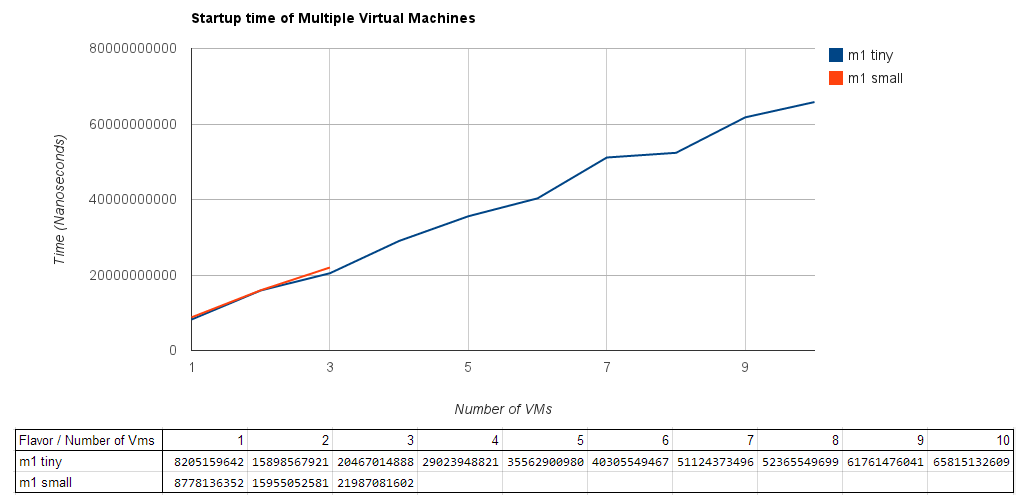
\includegraphics[scale=0.45]{multiple-server-launch-results}}
\caption{Execution times for Multiple Server Launch Experiment, averaged from 30 repetitions.}
\end{figure}

\begin{figure}[H]
\centering
\fbox{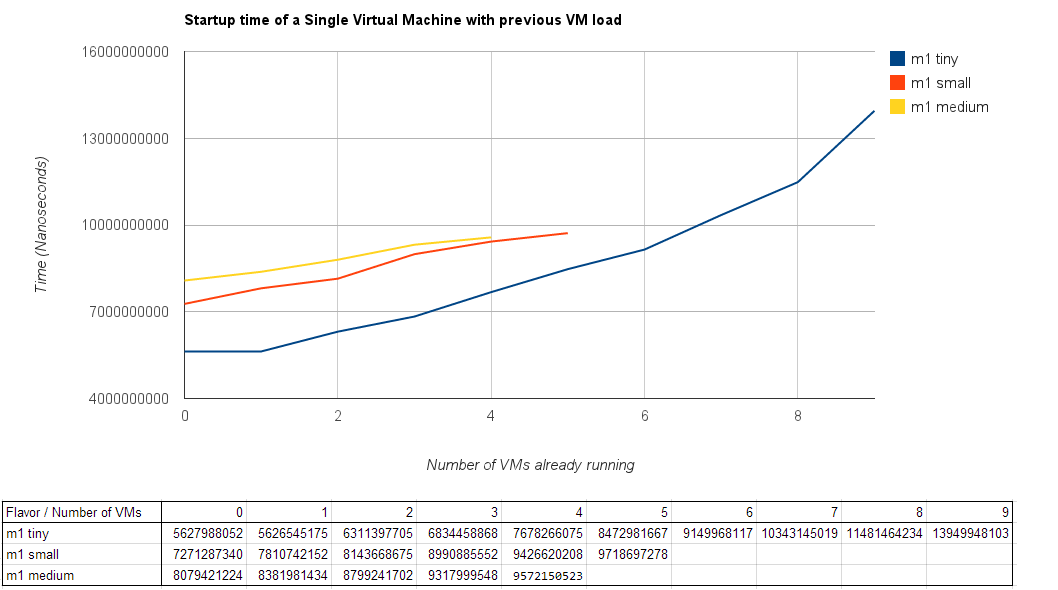
\includegraphics[scale=0.4]{single-vm-launch-results}}
\caption{Execution times for Single Server Launch Experiment, averaged from 30 repetitions.}
\end{figure}


The logs for these experiments can also be found in the /logs folder of the final submission, under the titles \textit{MultiServerStartupExperiment.log} and \textit{SingleServerStartupExperiment.log} respectively.

\textbf{Conclusion:}
Even though the data is limited, a number of conclusions can be drawn from each experiment. 
Firstly, from the first graph, we can see that OpenStack scales very well when starting virtual machines in parallel. The following graph shows how, from 1 VM to 10, adding 1 VM affects execution time, worked out by dividing the current (Current no. VMs) runtime by the previous runtime (Current no. VMs -1).  

\begin{figure}[H]
\centering
\fbox{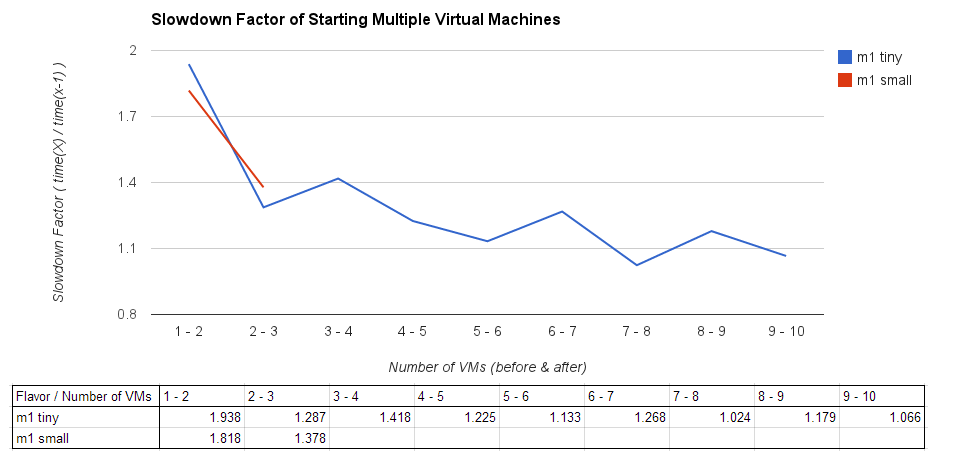
\includegraphics[scale=0.45]{slowdown-factor-multiple-launch}}
\caption{Slowdown factor of execution time from adding a VM for parallel launch}
\end{figure}

This diagram, using a concept similar to speedup\cite{speedup}, clearly indicates that OpenStack scales very well in terms of simultaneously launching Server VMs, even reducing the factor of slow down when VM load is higher. The gradient of the original curve shows this, it does not change greatly between 1 and 2 VMs, and 9 and 10. Similarly, flavor size does not appear to affect either the raw startup time, or in fact the factor of execution time increased, implying that OpenStack's ability to scale in terms of VM size is also very good. 
The second original graph shows similarly that OpenStack scales extremely well when creating single VMs with additional load on the Nova component. Starting VMs after already running more VMs does have a noticeable affect on performance however, as does flavor, but it is important to note that the gradient of each line is not dissimilar; this means that in terms of scaling, the execution slows down at a similar rate even when flavor size is larger. One statistic that is concerning is the change in gradient of the blue line, showing that the execution time difference between 9 and 10 VMs is relatively much larger than between 1 and 2 VMs. A slowdown diagram similar to that shown above illustrates this - the slowdown line for m1 tiny spikes as load increases:

\begin{figure}[H]
\centering
\fbox{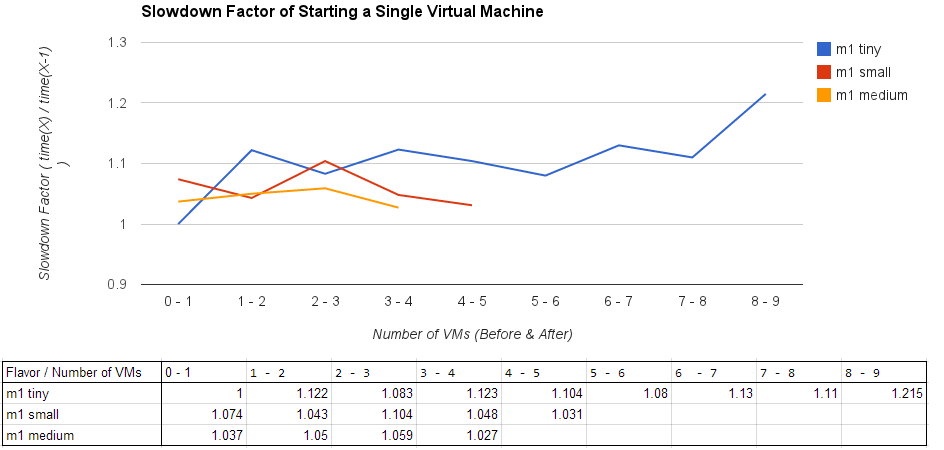
\includegraphics[scale=0.44]{slowdown-factor-single-launch}}
\caption{Slowdown factor of execution time from adding a VM load for single launch}
\end{figure}

Overall, these tests show that OpenStack has impressive scaling capabilities in terms of VM size, current VM load, and parallel VM launch. There are some issues, but further investigation on this would be required. 

\textbf{Resources:}
For the first part of the experiment, see \textit{MultiServerStartupExperiment.java} \& \textit{vm-startup-experiment.sh} in the final submission files. \\
For the second part, see \textit{SingleServerStartupExperiment.java} in the final submission files. 

\subsubsection{Experiment N4: Server Status Analysis}
\textbf{Introduction:}
Servers in OpenStack can have a number of Statuses, or States. When a Server is not active, there are a number of states it can be put in until it is needed again, in order to save energy, or compute capacity. In OpenStack, servers can be Paused, Suspended or Locked. 

\textbf{Aims, Considerations \& Metrics:}
Pausing a server stores it in RAM, whereas Suspending a server stores it on disk.\cite{nova-admin-server}. Locking the server just disallows certain operations to be performed on it. The idea behind this experiment is to see firstly which of these operations is fastest, and so generally preferred, and also whether the size of a Virtual Machine flavour has any effect on these operations. The metric to compare these will of course be execution time, averaged over a number of executions. 
I would expect suspending to be much slower than the other two, mainly due to its use of secondary storage. 

\textbf{Experiment Steps:} 
The experiment steps are as follows:
\begin{itemize}
\item For each Flavor:
	\begin{itemize}
	\item Create Server of size Flavor
	\item Perform each action couple {Pause, Unpause}, {Suspend, Resume}, {Lock, Unlock} and record times of each, REPETITIONS times.
	\item Take averages of these times 
	\end{itemize}
\end{itemize}
\textbf{Development \& Execution:}
Development of this experiment was relatively straightforward. The class \textit{ServerStatusPerformanceExperiment} was created, with code to perform the steps above, by looping through each flavor and repeatedly making calls to the Nova Extensions API to perform server admin actions such as pausing a server. A utility was created in the \textit{NovaUtils} class called \textit{waitForServerStatus} which allowed waiting for servers to change to the desired state, e.g. PAUSED, SUSPENDED. 

\textbf{Results:}
Below are the results of this experiment as a Bar chart. This shows the averaged execution time for each server operation, grouped by flavor size. 
\begin{figure}[H]
\centering
\fbox{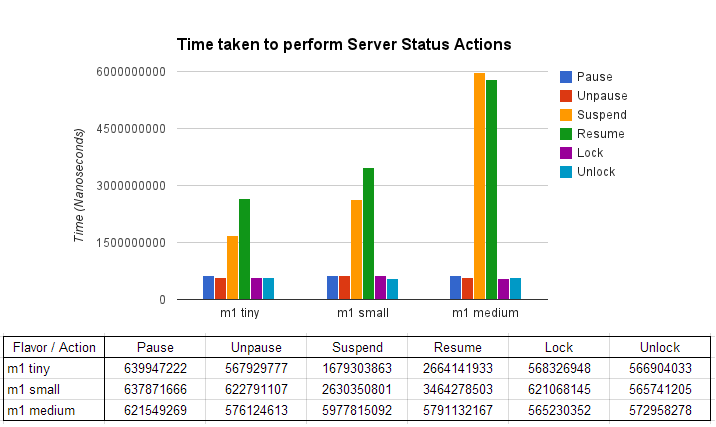
\includegraphics[scale=0.62]{server-status-results}}
\caption{Execution times of Server Admin Operations for different VM sizes}
\end{figure}
\textbf{Conclusion:}
As expected, these results firstly show that the Suspend \& Resume operations take a significant amount of time longer than the other operations, and this is most likely due to the overhead of writing to disk, especially with commodity hardware. The other actions only deal with operations in RAM, and this is known to be significantly faster.  \\
One surprising result here was the lack of increase in execution times in Locking \& Pausing operations as flavor size increases. As expected, Suspending \& Resuming a server takes much longer as flavor size increases, as more information is written to the disk. This pattern is not true however for the other operations, most likely due to writing to memory not having the same overhead as to disk. This of course has the disadvantage of being limited in capability; much larger VMs can be written to disk than can be written to RAM, especially in a system with a lot of load.  
We can conclude from this that, in many cases, locking and pausing a server is a much faster operation, but will still have an impact on RAM, and so Suspending a server may be the only option; in this case, one must be prepared for a long wait to write to disk, which appears to get exponentially larger as the VM size increases. 

\textbf{Resources:}
\textit{ServerStatusPerformanceExperiment}, \textit{NovaUtils}, \textit{ServerStatusPerformanceExperiment.log}